%!TEX root = ../crimson_throne_book_main.tex
% 2015-02-28
The companions wait fifteen minutes before returning to the warehouse. It looks like two Korvosan Guards are now patrolling the building on the outside. Quint, Puk and Balian wait for them to pass, before climbing up the wall to the roof. They make their way over the rooftop to the front of the building, above the office of Doctor Saulus. Puk keeps watch while Balian quietly pries away some of the wooden boards that cover the top of the building. A few moments later Quint and Puk slips into the doctor's workplace. Quint summons some light and goes over the writings on the desk. He puts the plague plan from Lost End next to them and compares the handwriting. There is no mistake: the same curls on the l's, the same 'dots' (or rather small lines) on the i's, and the same slant to the letters. In a drawer the bard also discovers a document that discusses the immunity to the plague in a certain part of the Varisian population, despite various attempts and experiments to get them sick. Then Quint's eye falls on a document with the doctor's name on it. Some letters stand out in the dim lightD v l s The office connects to the smaller upstairs {\itshape sick} ward, in which the patients weren't really sick, as Balian discovered earlier on. These must be the immune Varisian guinea pigs on which Saulus has been experimenting. Puk listens and hears one man walking around in the room. Balian joins his friends and draws his greatsword, while Quint signals to him that the enemy has to be taken alive. Puk pushes the handle down and clicks the door open, before slipping back in the dark corner. From inside the small sick ward he hears footsteps coming closer. A masked doctor stands off against the light in the background as he pushes open the door and peers into the dark of the office. Quint surprises the man with a {\itshape cacophonous call} , while Balian jumps up and hits him hard on the head with the pommel of his sword. The physician drops to the floor, unconscious. The patients in the room beyond do not react to this disturbance, they have obviously been drugged. The companions carry out the doctor, rejoin Sjo and make for the old fishery with their unconscious prisoner. They strip him of his clothes and discover a lot of strange vials and even a formula book in his leather coat. So, this man is an alchemist who uses chemistry to do his magic. Sjo throws a bucket of water in the man's face to wake him up, alchemy for beginners, lesson one.\\

At first the prisoner will only give up his name, Lennerd Brand. For the rest he feigns innocence. "We're here to help the people, that's all."\\

"Not a lot of help you are, then. I only saw dead leaving the hospital. Aren't you supposed to cure the sick? Well, I guess that is not what good old doctor Devils prescribes, is it?" Sjo spits.\\

"I can't help it that those people are just too far gone to be saved. We do our best. It's not like doctor Devils can perform miracles ... eh ... doctor Saulus, I mean."\\

"Haha, you stupid Urgathoan scum, nothing like a slip of the tongue to get to the truth", Sjo smiles as he burns the man in the leg with his power over fire. "Now spill the beans or suffer the consequences of your lies!"\\

"Here's the truth for you, you ignorant fool! Urgathoa's wrath will burn you all!" the doctor now scream madly.\\

"The only one who'll be burning with Urgathoa is you. Tell me, do you also dance around on skeletal legs in the afterlife when you're an Urgathoa hugger?" Sjo mocks.\\

"Just know that I'll be using these legs to dance on your eternally tortured soul. I give my life willingly to the Pallid Princess! She'll reserve a place of honor in her realm when I arrive after all we've achieved in this backwater city. Seldom has the queen of disease been served so well! Our success here will be the stuff of legends!" the doctor laughs.\\

"Tell us about your plans!"\\

"Never, I'll die before helping you."\\

"Well, I wouldn't say you'd have to die, that would be terribly inconvenient for both of us. Wouldn't you rather tell me all about the glory of Urgathoa right now?" Quint intervenes as he spins his verbal web of {\itshape fascination} again. The glare in the doctor's eyes tells him he is successful. "Now, if I can be so bold as to make a  {\itshape suggestion} , why don't you tell me what you know about Doctor Devil's plans." This time Quint's suggestion takes hold and the captured physician confesses: "Well, we arrived on that ship, the Delivery, but we got off before we reached the city, all except Rois. He was chosen as Urgathoa's champion, to sink the boat in the river mouth. We made it to shore and revealed ourselves a couple of days later as the 'doctors' who were supposed to fight the plague. We had to pretend that someone from Cheliax had teleported us in, you know, to explain how we got here so fast."\\

"And who are you working for?"\\

"I don't know, we get our orders from Doctor Devils and ... Lady Andaisin." The tone in the man's voice betrays that he is in awe of Urgathoa's highpriest.\\

"And where is she right now? Where are all of the doctor, actually?" Quint asks.\\

"There is a secret basement below the warehouse, if you switch a lever in the lift, it can take you down to our new temple! They say that this underground complex was used for smuggling in the past. The former owner of the building was none too happy when he had to give it up, {\itshape Arkomer} or something he was called. Anyway, that's where my brothers and sisters are, as is Lady Andaisin." "And what are you doing to those patients, especially the Varisian ones on the first floor?"\\

"It turns out that some Varisians are immune, we've been trying to find out how to get them sick, but nothing has worked so far. They are probably too stupid to realize that they should get sick, huhu, even rats know better", Lennerd replies with a cocky smile on his face as he stares at Balian. "Like that dimwit with the big sword, looks as stupid, but also as healthy as a horse."\\

Balian can't control himself and smacks the man in the head: "That will wipe that smirk of your face!" Unfortunately his aggressive action snaps the doctor out of Quint's suggestion. As it sinks in that he just gave away so many secrets, the man's face turns bitter. "What foul trickery did you throw over me? You will get no more answers out of me! Urgathoa damn you all to eternal hunger!"\\

"We have all we need from you, mister Brand. We'll be sure to tell your friends how cooperative you were. I'm sure they'll appreciate it", Sjo nods. "We'll be back for you later." At that Puk saps the man on the head, knocking him out again.\\

With only two to three hours left before sunrise, the companions know that they have to act quickly. Come morning, the physicians in the Hospice will discover that Saulus' office was broken into and that one of their own is missing. It will not be hard to link this break-in to the pseudodragon 'heroes' who were hanging around the backdoor earlier tonight. If they don't act immediately, the companions might have red Mantis assassins on their tails tomorrow. If there is still some element of surprise left, it is now!\\

Quint puts on the doctor's coat, hat and mask to make him look like one of the physicians. Sjo no longer objects to breaking the royal decree on this point, obviously the doctors are guilty of a worse crime: spreading the disease purposefully. The four heroes return to the warehouse. If they can bypass the ground floor, they will not have to face any innocent Korvosan guards or Gray Maidens. Not unless some of them are down in the underground temple as well, but then they won't be able to claim innocence anymore. Using the hole in the roof, the companions get back to the office on the first floor. Across from the sick room is the wooden elevator. Puk examines it and finds the switch that the doctor told them about. Pulling the ropes ever so quietly, Balian slowly descends the platform into the basement.\\

The way off the platform is blocked by a door. Puk listens at it but hears nothing. Time for some serious action! Then he\hyperref[fig:Entering-the-Temple-of-Urgathoa-516987053]{ pushes the door open } . \\

\begin{figure}[h]
	\centering
	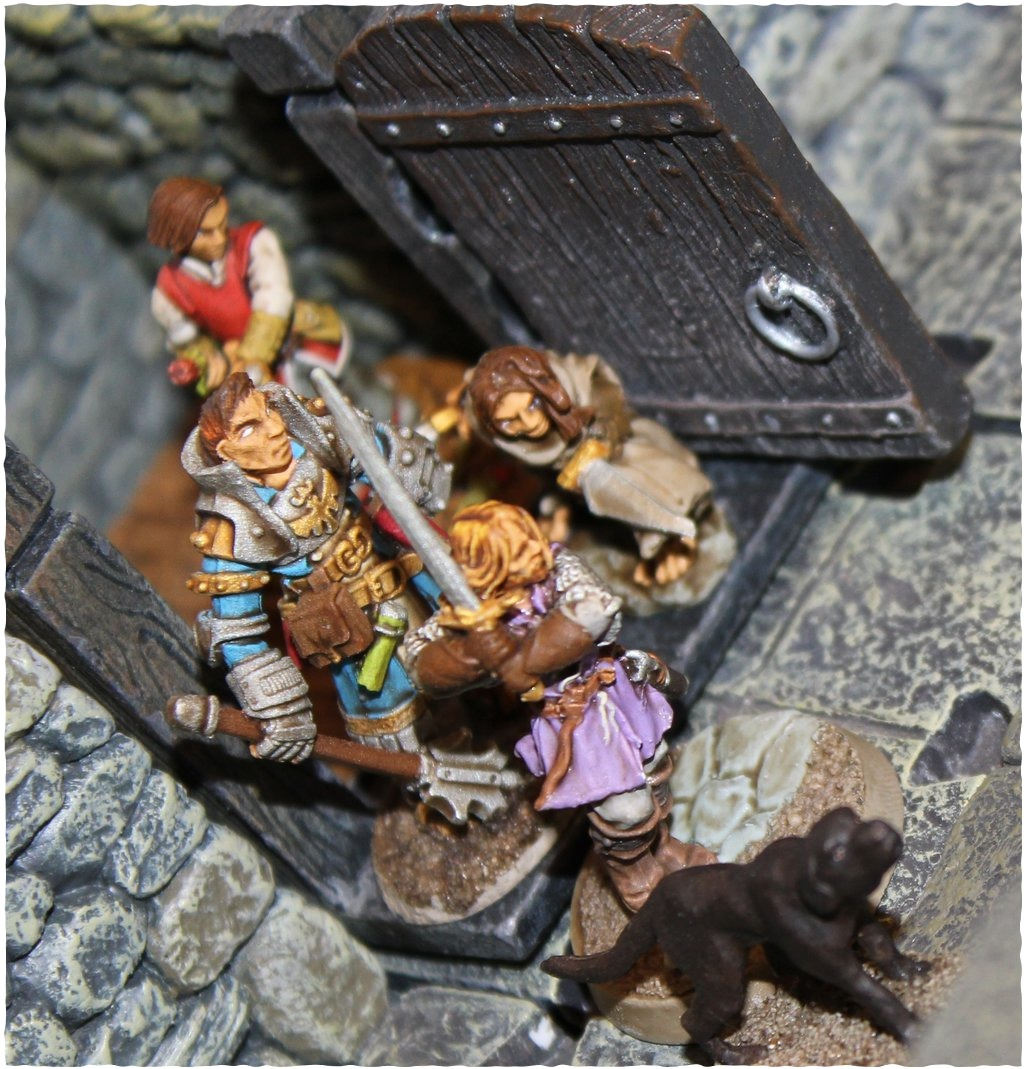
\includegraphics[width=0.4\textwidth]{images/Entering-the-Temple-of-Urgathoa-516987053_mod.jpg}
	\caption{Entering the Temple of Urgathoa}
	\label{fig:Entering-the-Temple-of-Urgathoa-516987053}
\end{figure}

